
%(BEGIN_QUESTION)
% Copyright 2010, Tony R. Kuphaldt, released under the Creative Commons Attribution License (v 1.0)
% This means you may do almost anything with this work of mine, so long as you give me proper credit

This thermocouple is installed improperly:

$$\includegraphics[width=15.5cm]{i00633x01.eps}$$

Identify the nature of the problem, and then calculate the millivoltage seen at the screw terminals of the temperature transmitter given the temperatures shown.  After that, calculate the temperature interpreted by the transmitter assuming it has cold junction compensation (CJC) enabled.

\underbar{file i00633}
%(END_QUESTION)





%(BEGIN_ANSWER)

The extension wire has been connected ``backwards'' to the thermocouple.  Yellow should connect to yellow, and red to red!

\vskip 10pt

Seeing how the {\it four} junctions' voltages interact is best done by drawing the circuit with each junction explicitly labeled as to polarity.  You will see that the process and reference (transmitter) junctions are aiding each other, and the two junctions formed at the head are opposing the first two (but aiding each other).  The formula for calculating voltage at the transmitter screw terminals then becomes:

$$V_{terminals} = V_{592^oC} + V_{23^oC} - V_{31^oC} - V_{31^oC}$$

$$V_{terminals} = 24.565 \hbox{ mV} + 0.919 \hbox{ mV} - 1.244 \hbox{ mV} - 1.244 \hbox{ mV}$$

$$V_{terminals} = 22.996 \hbox{ mV}$$

If the transmitter has CJC enabled, it will {\it add} 0.919 mV to compensate for the reference junction, making the interpreted (measurement junction) voltage equal to 23.915 mV.  This equates to 577 $^{o}$C, which is substantially cooler than the real process temperature.

%(END_ANSWER)





%(BEGIN_NOTES)

%INDEX% Measurement, temperature: thermocouple millivoltage interpretation

%(END_NOTES)


